\chapter{Performance Evaluation}
\label{chap:ch5}

This chapter presents a comprehensive performance evaluation of \texttt{rs\_ipc} against Python's standard inter-process communication mechanisms. The evaluation methodology is described in Section~\ref{sec:bench_methodology}, followed by scenario definitions in Section~\ref{sec:bench_scenarios}. Results are presented in Section~\ref{sec:bench_results}, with a detailed analysis of the copy versus zero-copy trade-off in Section~\ref{sec:copy_vs_zerocopy}. Section~\ref{sec:external_ipc} outlines planned comparisons with external IPC libraries. Rust-level microbenchmarks isolating synchronization overhead appear in Section~\ref{sec:rust_microbench}, and Section~\ref{sec:bench_discussion} synthesizes the findings.

\section{Benchmarking Methodology}
\label{sec:bench_methodology}

\subsection{Hardware and Software Environment}

All measurements were collected on a single workstation to eliminate network variability and ensure reproducible results. Table~\ref{tab:environment} summarizes the test environment.

\begin{table}[htbp]
    \centering
    \caption{Benchmark hardware and software environment.}
    \label{tab:environment}
    \begin{tabular}{ll}
        \hline
        \textbf{Component} & \textbf{Specification} \\
        \hline
        CPU & AMD Ryzen 7 7700, 8 cores / 16 threads \\
        Clock & 3.8~GHz base, 5.4~GHz boost \\
        L1 Data Cache & 32~KiB per core \\
        L2 Cache & 1~MiB per core \\
        L3 Cache & 32~MiB shared \\
        Memory & 32~GiB DDR5 \\
        Operating System & Arch Linux \\
        Kernel & Linux 7.0.9 \\
        Python & 3.14.5 \\
        Rust Toolchain & 1.95.0 \\
        \hline
    \end{tabular}
\end{table}

\subsection{Measurement Approach}

The benchmark framework employs true multiprocessing via Python's \texttt{spawn} start method, ensuring each participant runs in a separate process with its own address space. This reflects realistic deployment conditions where IPC is necessary precisely because threads cannot share state freely due to the GIL.

Startup synchronization uses a \texttt{multiprocessing.Barrier} so that all writer and reader processes begin their measurement loops simultaneously. Latency is measured end-to-end: the writer embeds a \texttt{time.time()} timestamp in each message immediately before transmission, and the reader computes the difference upon receipt. This captures the full IPC path including serialization, synchronization, memory transfer, and deserialization.

\subsection{Payload}

The primary payload is a \texttt{MockPipeData} structure containing three NumPy arrays of shape $640 \times 480 \times 3$ (unsigned 8-bit integers), representative of a triple-channel video frame from a computer vision pipeline. After pickle serialization, this payload occupies approximately 2.76~MB, corresponding to a single 640$\times$480 RGB frame---a common resolution in autonomous driving and robotics applications.

For size-scaling experiments, raw byte buffers of 1, 2, 4, 8, 16, and 32~MB are used to isolate the effect of payload size from serialization overhead.

\subsection{Metrics}

Four metrics characterize IPC performance:

\begin{itemize}
    \item \textbf{Median latency (p50)}: The 50th percentile of end-to-end message delivery time in milliseconds. Represents typical-case performance.

    \item \textbf{Tail latency (p99)}: The 99th percentile latency. Critical for real-time systems where worst-case behavior determines system feasibility.

    \item \textbf{Throughput}: Total bytes transferred divided by wall-clock duration, expressed in MB/s. Captures sustained transfer rate including synchronization overhead.

    \item \textbf{Determinism ratio}: Defined as $\text{p99} / \text{p50}$. A ratio of 1.0 indicates perfectly predictable latency; higher values indicate jitter. For real-time applications, predictable latency is often more valuable than lowest average latency.
\end{itemize}

\subsection{Statistical Methodology}

Each scenario executes 200 iterations for the standard payload size, with iteration counts scaled down for larger payloads to maintain reasonable execution time (e.g., approximately 12 iterations for 32~MB messages). Percentiles are computed using NumPy's percentile function over all received messages per reader process. When multiple readers participate, the reported p50 and p99 represent the arithmetic mean of per-reader percentiles. No warmup iterations are discarded; the barrier synchronization ensures that all processes begin measurement simultaneously, and the first few iterations capture cold-start behavior that is relevant to real deployments.

\subsection{Backends Under Test}

Five IPC backends are evaluated:

\begin{itemize}
    \item \textbf{RsIpc (zerocopy)}: The writer acquires a write guard and invokes \texttt{pickle.dump(obj, guard)}, serializing directly into shared memory via the Python buffer protocol. The reader acquires a read guard and calls \texttt{pickle.loads(guard)}, deserializing directly from shared memory. No intermediate copies are created.

    \item \textbf{RsIpc (copy)}: The writer serializes with \texttt{pickle.dumps(obj)} into a temporary Python bytes object, then calls \texttt{shm.write(bytes)} which performs a single \texttt{memcpy} into shared memory. The reader receives a Rust-allocated copy of the shared memory contents and deserializes from that copy.

    \item \textbf{multiprocessing.Queue}: Python's standard thread-safe, process-safe queue. Internally uses pipes with a background feeder thread for serialization. Bounded to size 1 for fair comparison with fixed-size shared memory slots.

    \item \textbf{multiprocessing.Pipe}: Low-level bidirectional connection using OS pipes. In multi-reader scenarios, a \texttt{multiprocessing.Lock} serializes writer access to prevent interleaved messages.

    \item \textbf{multiprocessing.shared\_memory (MpShm)}: Python's native shared memory module, supplemented with manual \texttt{multiprocessing.Lock} and \texttt{multiprocessing.Condition} for synchronization. This backend replicates what a developer would build using only the standard library, and serves as a direct comparison point for the synchronization quality of \texttt{rs\_ipc}.
\end{itemize}


\section{Scenarios}
\label{sec:bench_scenarios}

Four scenario categories evaluate different aspects of IPC performance:

\begin{itemize}
    \item \textbf{Latency (1:1)}: A single producer communicates with a single consumer. This baseline scenario isolates raw IPC overhead without contention or fan-out effects.

    \item \textbf{Scalability (1:10)}: One writer distributes data to ten readers simultaneously. This pattern represents a camera feed shared among multiple processing pipelines (e.g., object detection, lane tracking, depth estimation running in parallel).

    \item \textbf{Contention (10:1)}: Ten writers send data to a single reader. This fan-in pattern models multiple sensors feeding a single aggregator or fusion module.

    \item \textbf{Size scaling (1--32~MB)}: Single producer--consumer communication with varying payload sizes, from 1~MB to 32~MB. This reveals how performance degrades as messages approach and exceed the L3 cache capacity (32~MiB on the test system).
\end{itemize}


\section{Results: Comparison with Python Standard Library}
\label{sec:bench_results}

\subsection{Latency and Tail Latency}
\label{subsec:latency_results}

Table~\ref{tab:latency_results} presents the complete latency and throughput results across the three core scenarios. The determinism ratio (p99/p50) quantifies latency predictability.

\begin{table}[htbp]
    \centering
    \caption{Latency and throughput results across core scenarios (2.76~MB payload).}
    \label{tab:latency_results}
    \resizebox{\textwidth}{!}{%
    \begin{tabular}{llrrrr}
        \hline
        \textbf{Scenario} & \textbf{Backend} & \textbf{p50 (ms)} & \textbf{p99 (ms)} & \textbf{MB/s} & \textbf{Determinism} \\
        \hline
        \multirow{5}{*}{Latency (1:1)}
        & RsIpc (zerocopy) & 0.84 & 1.12 & 6,104 & 1.33 \\
        & RsIpc (copy) & 0.19 & 0.22 & 25,886 & 1.13 \\
        & MpQueue & 1.42 & 2.37 & 2,172 & 1.67 \\
        & MpPipe & 0.72 & 1.00 & 3,889 & 1.39 \\
        & MpShm & 0.84 & 1.01 & 6,243 & 1.20 \\
        \hline
        \multirow{5}{*}{Scalability (1:10)}
        & RsIpc (zerocopy) & 1.98 & 2.37 & 2,513 & 1.20 \\
        & RsIpc (copy) & 2.96 & 5.36 & 1,602 & 1.81 \\
        & MpQueue & 6.63 & 11.49 & 471 & 1.73 \\
        & MpPipe & 4.32 & 5.30 & 345 & 1.23 \\
        & MpShm & 8.95 & 10.95 & 523 & 1.22 \\
        \hline
        \multirow{5}{*}{Contention (10:1)}
        & RsIpc (zerocopy) & 0.83 & 1.11 & 6,096 & 1.33 \\
        & RsIpc (copy) & 1.85 & 4.50 & 15,233 & 2.43 \\
        & MpQueue & 2.01 & 2.49 & 1,712 & 1.24 \\
        & MpPipe & 0.74 & 1.16 & 3,787 & 1.57 \\
        & MpShm & 2.01 & 34.71 & 5,021 & 17.30 \\
        \hline
    \end{tabular}%
    }
\end{table}

In the baseline 1:1 scenario, RsIpc (copy) achieves the lowest median latency at 0.19~ms---7.3$\times$ faster than \texttt{multiprocessing.Queue} and 3.8$\times$ faster than MpPipe. RsIpc (zerocopy) and MpShm show similar p50 values (0.84~ms), as both ultimately rely on shared memory for data transfer. The critical difference emerges in multi-participant scenarios.

Figure~\ref{fig:tail_latency} visualizes the p99 tail latency across scenarios on a logarithmic scale.

\begin{figure}[htbp]
    \centering
    
\includegraphics[width=\textwidth]{./figures/01_tail_latency.png}
    \caption{Tail latency (p99) comparison across scenarios. Logarithmic scale emphasizes the order-of-magnitude differences under contention. MpShm exhibits catastrophic tail latency (34.71~ms) in the 10:1 contention scenario.}
    \label{fig:tail_latency}
\end{figure}

The most striking result appears in the contention scenario (10:1): MpShm produces a p99 of 34.71~ms---a 17.3$\times$ ratio over its median. This occurs because Python's \texttt{multiprocessing.Condition} uses polling with 10~ms timeouts (the minimum granularity of \texttt{Condition.wait(timeout)}), causing writers to occasionally sleep for a full timeout interval when the condition notification arrives between polls. The futex-based implementation in \texttt{rs\_ipc} avoids this pathology entirely: the spin-then-sleep strategy described in Chapter~\ref{chap:ch4} ensures sub-millisecond wakeup latency.

\subsection{Determinism and Predictability}
\label{subsec:determinism_results}

Figure~\ref{fig:determinism} presents the determinism ratio (p99/p50) for each backend across the core scenarios.

\begin{figure}[htbp]
    \centering
    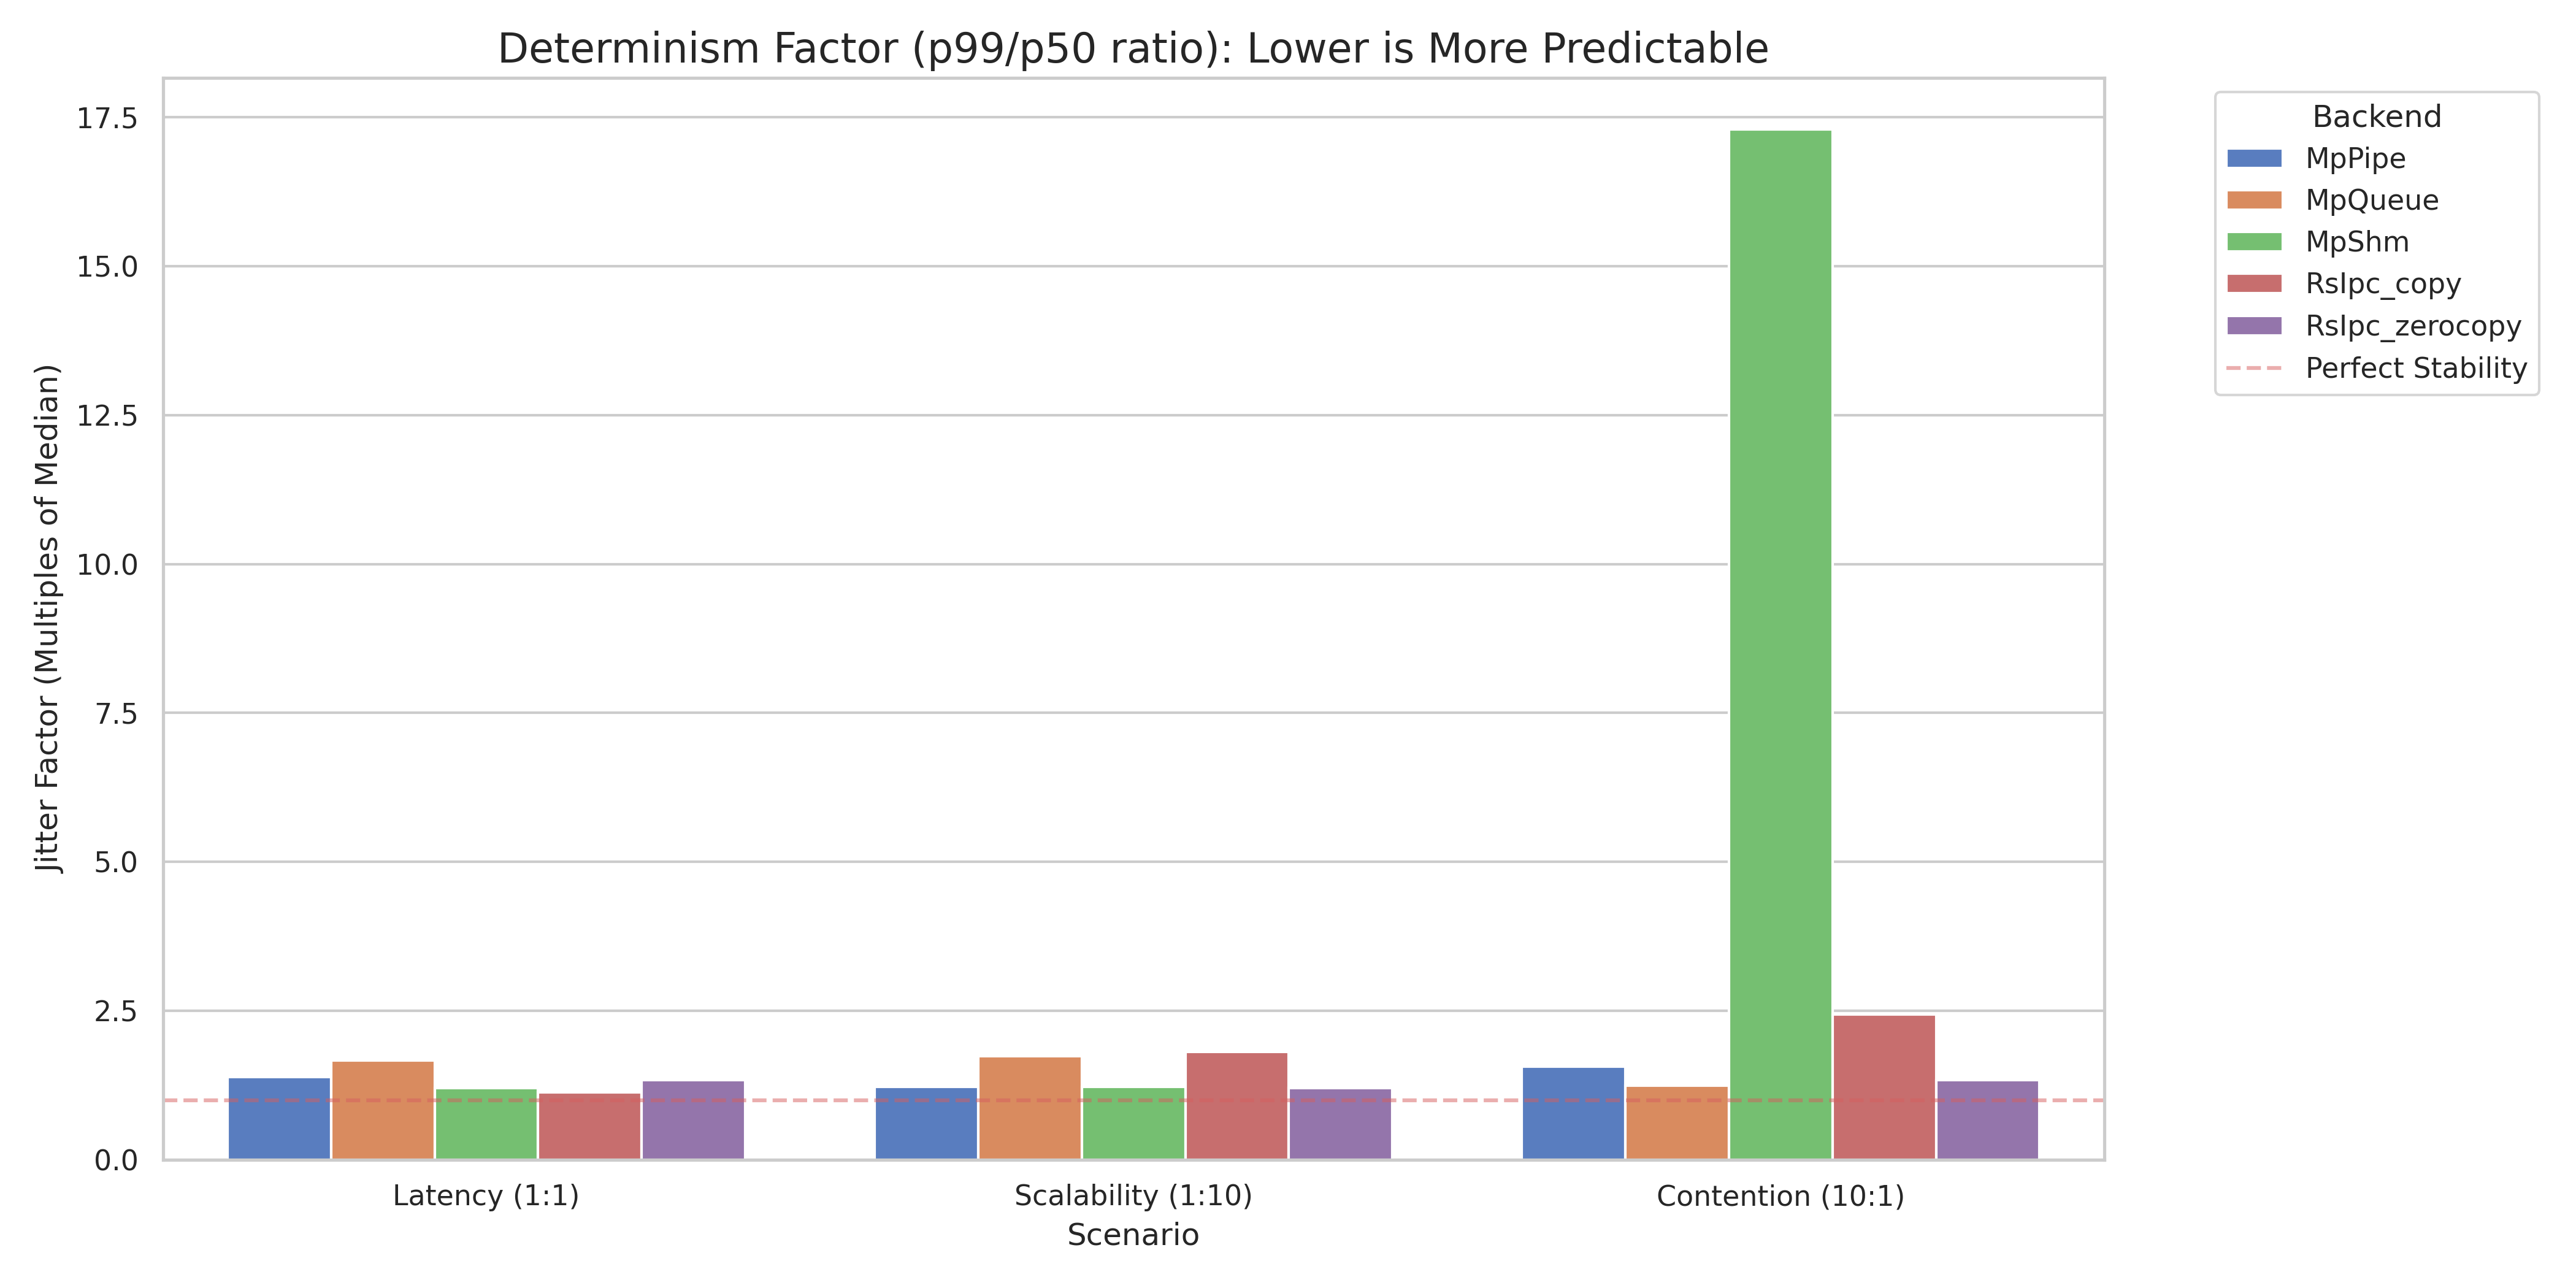
\includegraphics[width=\textwidth]{./figures/02_determinism.png}
    \caption{Determinism factor (p99/p50 ratio) across scenarios. A ratio of 1.0 represents perfectly predictable latency. RsIpc (zerocopy) maintains a ratio below 1.4 in all scenarios, while MpShm degrades to 17.3$\times$ under contention.}
    \label{fig:determinism}
\end{figure}

RsIpc (zerocopy) demonstrates the most consistent behavior, maintaining a determinism ratio below 1.4 across all three scenarios. This stability stems from the futex-based synchronization: the combination of spin-waiting (up to 1000 iterations in \texttt{SharedCondvar}) and direct kernel notification via \texttt{futex\_wake\_all} ensures bounded wakeup latency regardless of contention level.

RsIpc (copy) exhibits higher variance under contention (2.43$\times$) due to the interaction between multiple writers contending for the \texttt{FutexLock} and the three-state lock protocol. When the lock transitions to the \texttt{CONTENDED} state, waiting writers must perform a futex system call, introducing kernel scheduling latency. Nevertheless, this remains well below the 17.3$\times$ ratio observed with MpShm.

For real-time applications, predictable latency is often more critical than minimal average latency. A system with p50 = 2~ms and p99 = 3~ms (ratio 1.5) is preferable to one with p50 = 1~ms and p99 = 35~ms (ratio 35) because the former permits tighter deadline budgeting.

\subsection{Throughput and Efficiency}
\label{subsec:throughput_results}

Figure~\ref{fig:efficiency} shows the efficiency score (throughput in MB/s divided by median latency in ms) for each backend and scenario.

\begin{figure}[htbp]
    \centering
    
\includegraphics[width=\textwidth]{./figures/03_efficiency.png}
    \caption{Architectural efficiency: throughput (MB/s) per millisecond of median latency. Higher values indicate better utilization of the available bandwidth relative to synchronization cost. RsIpc (copy) dominates in the 1:1 scenario due to its minimal lock hold time.}
    \label{fig:efficiency}
\end{figure}

In the 1:1 scenario, RsIpc (copy) achieves 25,886~MB/s throughput---equivalent to approximately 25.3~GB/s, approaching the theoretical DDR5 memory bandwidth of the test system. This result demonstrates that the synchronization overhead (futex lock acquisition, sequence increment) is negligible compared to the \texttt{memcpy} cost: a single 2.76~MB copy completes in under 200~\textmu s.

In the scalability scenario (1:10), RsIpc (zerocopy) achieves the highest throughput (2,513~MB/s) among all backends. This advantage arises because the zerocopy mode allows multiple readers to access shared memory concurrently without requiring per-reader copies, while the copy mode must serialize each reader's access through the write lock (since the write overwrites the shared buffer). The throughput advantage of RsIpc over \texttt{multiprocessing.Queue} (5.3$\times$) and \texttt{multiprocessing.Pipe} (7.3$\times$) in this scenario reflects the fundamental overhead of pipe-based communication: each message must traverse the kernel pipe buffer for each reader independently.

\subsection{Message Size Scaling}
\label{subsec:size_scaling_results}

Table~\ref{tab:size_scaling} presents throughput across message sizes for the 1:1 scenario, and Figure~\ref{fig:size_scaling} visualizes the scaling behavior.

\begin{table}[htbp]
    \centering
    \caption{Throughput (MB/s) by message size in the 1:1 scenario.}
    \label{tab:size_scaling}
    \begin{tabular}{lrrrrr}
        \hline
        \textbf{Size} & \textbf{RsIpc (zc)} & \textbf{RsIpc (cp)} & \textbf{MpQueue} & \textbf{MpPipe} & \textbf{MpShm} \\
        \hline
        1~MB  & 21,014 & 3,341 & 2,323 & 3,624 & 3,150 \\
        2~MB  & 23,283 & 3,396 & 1,856 & 3,746 & 3,305 \\
        4~MB  & 26,246 & 19,378 & 2,328 & 3,693 & 18,200 \\
        8~MB  & 25,975 & 14,974 & 2,339 & 3,819 & 18,566 \\
        16~MB & 17,814 & 7,676 & 2,313 & 3,644 & 10,312 \\
        32~MB & 3,449 & 2,322 & 1,533 & 1,560 & 3,427 \\
        \hline
    \end{tabular}
\end{table}

\begin{figure}[htbp]
    \centering
    
\includegraphics[width=\textwidth]{./figures/04_size_scaling.png}
    \caption{Throughput versus message size (1:1 scenario, log-scale x-axis). RsIpc (zerocopy) maintains superior throughput up to 16~MB before degrading at 32~MB as the working set exceeds L3 cache capacity.}
    \label{fig:size_scaling}
\end{figure}

Three distinct regimes emerge from the size-scaling data:

\textbf{Small messages (1--2~MB)}: RsIpc (zerocopy) achieves 21,000--23,000~MB/s, far exceeding all other backends. At these sizes, the entire message fits within the L3 cache, and the zerocopy path---which writes directly into shared memory without an intermediate buffer---avoids the cache pollution that a temporary allocation would cause. MpPipe and MpQueue maintain consistent but low throughput (2,300--3,700~MB/s), bounded by kernel pipe buffer management overhead.

\textbf{Medium messages (4--8~MB)}: Both RsIpc (zerocopy) at 26,000~MB/s and the shared-memory-based backends (RsIpc copy, MpShm) at 14,000--19,000~MB/s achieve high throughput. The working set still fits within the L3 cache (32~MiB), enabling efficient streaming from the write buffer. MpPipe and MpQueue remain capped by kernel copy overhead.

\textbf{Large messages (16--32~MB)}: Performance degrades sharply for all shared-memory backends. At 32~MB, the working set equals the L3 cache size, causing cache thrashing: the write and read of a single message evict the entire cache contents. RsIpc (zerocopy) and MpShm converge to similar throughput (3,427--3,449~MB/s), as both reduce to a single \texttt{memcpy}-equivalent operation bounded by DRAM bandwidth. Pipe-based mechanisms (MpQueue, MpPipe) degrade further due to additional kernel-mediated copies.


\section{Analysis: Copy vs.\ Zero-Copy Trade-off}
\label{sec:copy_vs_zerocopy}

The benchmark results reveal a counterintuitive finding: the ``copy'' mode of \texttt{rs\_ipc} consistently outperforms the ``zerocopy'' mode in latency for pickle-based workloads (0.19~ms vs.\ 0.84~ms in the 1:1 scenario). This section analyzes the root cause and identifies the conditions under which each mode is optimal.

\subsection{Critical Section Analysis}

The fundamental difference between the two modes lies in their lock hold duration. Table~\ref{tab:critical_section} summarizes the execution paths.

\begin{table}[htbp]
    \centering
    \caption{Critical section comparison between copy and zerocopy modes.}
    \label{tab:critical_section}
    \begin{tabular}{lll}
        \hline
        \textbf{Phase} & \textbf{Copy Mode} & \textbf{Zerocopy Mode} \\
        \hline
        1. Serialize & \texttt{pickle.dumps(obj)} & (deferred to step 3) \\
          & $\sim$800~\textmu s, no lock held & \\
        2. Acquire lock & \texttt{start\_write()} & \texttt{write\_guard()} \\
          & via \texttt{FutexLock} & via \texttt{FutexLock} \\
        3. Transfer data & single \texttt{memcpy} & \texttt{pickle.dump(obj, guard)} \\
          & $\sim$2~\textmu s & $\sim$800~\textmu s, hundreds of \\
          & & incremental \texttt{.write()} calls \\
        4. Publish & sequence increment & sequence increment \\
        5. Release lock & drop guard & drop guard \\
        \hline
        \textbf{Lock hold time} & $\sim$2~\textmu s & $\sim$800~\textmu s \\
        \hline
    \end{tabular}
\end{table}

In copy mode, serialization occurs entirely outside the critical section. The writer calls \texttt{pickle.dumps(obj)} to produce a byte string in the Python heap (approximately 800~\textmu s for a 2.76~MB payload), then acquires the writer mutex and performs a single \texttt{ptr::copy\_nonoverlapping} to transfer the pre-serialized data into shared memory. The lock is held for approximately 2~\textmu s---just the duration of one \texttt{memcpy}.

In zerocopy mode, the writer first acquires the lock via \texttt{write\_guard()}, then calls \texttt{pickle.dump(obj, guard)}. The pickle protocol serializes the object through hundreds of incremental \texttt{.write()} calls to the guard's buffer protocol interface. Each call crosses the Python-to-Rust FFI boundary, performs a bounds check, and executes a small \texttt{memcpy} into shared memory. The lock is held throughout this entire process---approximately 800~\textmu s.

The ratio of lock hold times is approximately 400$\times$, which directly impacts contention: in multi-reader scenarios, readers must wait for the writer to release the mutex before accessing updated data.

\subsection{When Each Mode Excels}

Despite its higher latency in pickle-based workloads, the zerocopy mode offers advantages in specific use cases:

\begin{itemize}
    \item \textbf{Pre-serialized data}: When the payload is already a contiguous byte buffer (e.g., a raw NumPy array or a pre-encoded video frame), the zerocopy write path performs a single large \texttt{memcpy} identical to copy mode, but avoids allocating a temporary buffer. The size-scaling results confirm this: at 1~MB with raw byte payloads, RsIpc (zerocopy) achieves 21,014~MB/s versus 3,341~MB/s for copy mode.

    \item \textbf{Memory-constrained environments}: Copy mode requires allocating a temporary buffer equal to the serialized message size. For large payloads or systems with limited memory headroom, zerocopy eliminates this allocation entirely.

    \item \textbf{Fan-out patterns}: In the 1:10 scalability scenario, zerocopy achieves 1.85$\times$ higher throughput than copy mode (2,513 vs.\ 1,602~MB/s). Multiple readers can access the shared memory region concurrently through read guards, whereas copy mode incurs per-reader overhead.
\end{itemize}

The recommendation for application developers is clear: use copy mode for pickle-based workloads where latency is the primary concern, and zerocopy mode for pre-serialized data (raw arrays, encoded frames) or memory-constrained multi-reader scenarios where throughput dominates.


\section{Comparison with External IPC Libraries}
\label{sec:external_ipc}

A comprehensive comparison with external IPC libraries beyond Python's standard library is planned as future work. The following systems are targeted for evaluation:

\begin{itemize}
    \item \textbf{ZeroMQ}: Using PAIR sockets with the IPC transport, representing a mature general-purpose messaging library with batching and zero-copy optimizations.
    \item \textbf{nanomsg / nng}: A lightweight messaging library with similar socket abstractions but simpler internals.
    \item \textbf{Unix domain sockets}: Raw socket communication without a messaging framework, establishing the baseline for kernel-mediated IPC.
    \item \textbf{Rust ipc-channel}: Mozilla's Rust-native IPC library, evaluating the overhead of a Rust-to-Rust path through Python bindings.
\end{itemize}

These comparisons will use the same methodology described in Section~\ref{sec:bench_methodology}, with the 2.76~MB payload and both the 1:1 and 1:10 scenarios as primary evaluation points. The focus will be on latency and throughput positioning: \texttt{rs\_ipc} targets a niche between raw shared memory (maximum performance, no safety) and general-purpose messaging (convenience, higher overhead).


\section{Rust-Level Microbenchmarks}
\label{sec:rust_microbench}

To isolate the cost of the Rust synchronization layer from Python/PyO3/pickle overhead, Criterion microbenchmarks measure raw write throughput at the Rust level using a 1~MB payload.

\subsection{Benchmark Configuration}

Three benchmark functions evaluate different synchronization costs:

\begin{itemize}
    \item \textbf{\texttt{pure\_write}}: Writes 1~MB to shared memory with \texttt{target\_read\_count = 0} and no registered readers. Measures the raw write path: mutex acquisition, \texttt{memcpy}, sequence increment, mutex release.

    \item \textbf{\texttt{write\_no\_wait\_with\_reader}}: Same configuration as \texttt{pure\_write}, but with one registered reader consuming messages on a background thread. The writer does not wait for consumption (\texttt{target\_read\_count = 0}), so this measures the cost of concurrent reader access on the write path.

    \item \textbf{\texttt{write\_waiting\_with\_N\_readers}}: Configures \texttt{target\_read\_count = N} with $N$ active reader threads. The writer blocks in \texttt{start\_write()} until all $N$ readers have consumed the previous message. This measures the full synchronization cost including condvar signaling and wakeup latency.
\end{itemize}

Each benchmark uses Criterion's default configuration with 50 samples and 2-second measurement windows per sample.

\subsection{Expected Scaling Behavior}

The write-with-readers benchmarks reveal the synchronization cost as a function of reader count. With \texttt{target\_read\_count = N}, the writer must wait for the \texttt{data\_consumed} counter (packed in the \texttt{ReadersStateCount} atomic, as described in Chapter~\ref{chap:ch4}) to reach $N$ before proceeding. Each reader increments this counter upon completing its read, triggering a \texttt{futex\_wake\_all} on the writer's condvar.

The expected latency increase per additional reader is bounded by:
\begin{enumerate}
    \item The read duration (1~MB \texttt{memcpy} $\approx$ 100--200~\textmu s per reader, parallelized across cores).
    \item One \texttt{futex\_wake} system call per reader completion ($\approx$ 1~\textmu s each).
    \item The writer's spin-wait or \texttt{futex\_wait} to observe the counter update.
\end{enumerate}

Since readers operate concurrently, the total wait time scales with the slowest reader rather than the sum of all readers---a consequence of the partial-blocking design described in Section~\ref{sec:sync} of Chapter~\ref{chap:ch2}. However, cache contention on the \texttt{ReadersStateCount} atomic increases linearly with reader count due to the MESI invalidation traffic described in Section~\ref{subsec:false_sharing} of Chapter~\ref{chap:ch2}.


\section{Discussion}
\label{sec:bench_discussion}

\subsection{Where rs\_ipc Excels}

The benchmark results identify three areas of clear advantage for \texttt{rs\_ipc}:

\textbf{Multi-reader scalability}: In the 1:10 scenario, RsIpc (zerocopy) achieves 5.3$\times$ higher throughput than \texttt{multiprocessing.Queue} and 4.8$\times$ higher than MpShm. The lock-free version checking mechanism (described in Chapter~\ref{chap:ch4}) allows readers to detect new messages without acquiring any lock, reducing contention on the critical path.

\textbf{Tail latency predictability}: RsIpc maintains determinism ratios below 2.5$\times$ in all scenarios, while MpShm degrades catastrophically (17.3$\times$) under writer contention. The futex-based synchronization provides bounded wakeup latency that Python's condition variable polling cannot match.

\textbf{Large payload throughput}: For pre-serialized data in the 4--8~MB range, RsIpc (zerocopy) achieves 25,000--26,000~MB/s---approximately 7$\times$ higher than pipe-based mechanisms and 1.4$\times$ higher than MpShm.

\subsection{Limitations}

\textbf{Copy mode paradox}: For pickle-based workloads, the ``copy'' mode outperforms ``zerocopy'' in latency because pickle serialization holds the writer mutex for the entire serialization duration in zerocopy mode. This is inherent to the buffer-protocol approach and cannot be resolved without changing the pickle protocol or pre-serializing data.

\textbf{32~MB degradation}: At payload sizes equal to or exceeding the L3 cache (32~MiB), all shared-memory backends converge to similar performance, bounded by DRAM bandwidth. The synchronization advantages of \texttt{rs\_ipc} become irrelevant when memory subsystem throughput is the bottleneck.

\textbf{Platform restriction}: The futex-based synchronization is Linux-specific. Portability to other operating systems would require alternative synchronization backends (e.g., Windows \texttt{WaitOnAddress}, macOS \texttt{os\_unfair\_lock}), potentially with different performance characteristics.

\subsection{Implications for System Design}

The results suggest the following guidelines for developers choosing an IPC strategy:

\begin{enumerate}
    \item For single-producer, single-consumer pipelines with pickle-based data: \texttt{rs\_ipc} copy mode offers 7$\times$ lower latency than \texttt{multiprocessing.Queue} with minimal API complexity.

    \item For fan-out architectures (one camera, multiple consumers): \texttt{rs\_ipc} zerocopy mode provides the best combination of throughput and predictability, with the added benefit of concurrent reader access.

    \item For latency-critical paths with raw byte data (pre-encoded frames, NumPy arrays): \texttt{rs\_ipc} zerocopy mode achieves true zero-copy semantics with throughput approaching memory bandwidth limits.

    \item When predictable worst-case latency matters more than average performance: \texttt{rs\_ipc}'s determinism advantage (1.2--1.4$\times$ ratio vs.\ up to 17$\times$ for MpShm) enables tighter deadline budgets in real-time systems.
\end{enumerate}
